
\begin{figure}
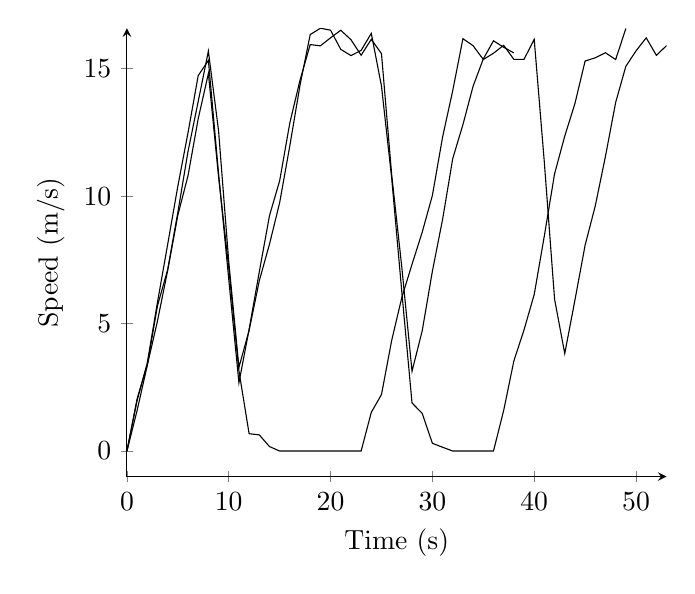
\begin{tikzpicture}
\begin{axis}[
legend style={anchor=west},
axis x line=bottom,
axis y line=left,
ymin=-1,
xlabel=Time (s),
ylabel=Speed (m/s),
]
\addplot[] coordinates {
(0, 0.0)
(1, 1.59303435794)
(2, 3.36218318495)
(3, 5.1013594048)
(4, 7.0818780936)
(5, 9.24984151847)
(6, 10.8010152579)
(7, 13.033315911)
(8, 14.8056760005)
(9, 10.7584669005)
(10, 7.18891576149)
(11, 3.14549959745)
(12, 0.68044636141)
(13, 0.634226804167)
(14, 0.176466034343)
(15, 0.0)
(16, 0.0)
(17, 0.0)
(18, 0.0)
(19, 0.0)
(20, 0.0)
(21, 0.0)
(22, 0.0)
(23, 0.0)
(24, 1.51716525696)
(25, 2.21479517603)
(26, 4.33440314714)
(27, 6.02566269742)
(28, 7.3239630102)
(29, 8.58397881987)
(30, 10.0265533377)
(31, 12.3112598381)
(32, 14.1437834794)
(33, 16.1747326728)
(34, 15.8993714419)
(35, 15.3583040629)
(36, 15.6032261398)
(37, 15.9151511645)
(38, 15.36553874)
(39, 15.3638390096)
(40, 16.1494877051)
(41, 11.3003394455)
(42, 5.95893366755)
(43, 3.82454691462)
(44, 5.92035971473)
(45, 8.074132627)
(46, 9.61958684849)
(47, 11.5639178525)
(48, 13.6740866971)
(49, 15.0909012548)
(50, 15.6969450434)
(51, 16.2070702747)
(52, 15.5215074183)
(53, 15.9040624156)
};
\addplot[] coordinates {
(0, 0.0)
(1, 1.98205558845)
(2, 3.46252841176)
(3, 5.83488941425)
(4, 8.10146303789)
(5, 10.3913908594)
(6, 12.4854218517)
(7, 14.7248938272)
(8, 15.3201615499)
(9, 10.8900730615)
(10, 6.73963570815)
(11, 2.67775828797)
(12, 4.77427282683)
(13, 7.02769474643)
(14, 9.23059956687)
(15, 10.6018223438)
(16, 12.8740622143)
(17, 14.5463010511)
(18, 15.9440976221)
(19, 15.8934330559)
(20, 16.2102697277)
(21, 16.5050917872)
(22, 16.137223762)
(23, 15.5247038498)
(24, 16.1502788253)
(25, 15.5872180569)
(26, 10.8487136246)
(27, 7.19761681876)
(28, 3.12860720255)
(29, 4.7142662389)
(30, 7.05352267995)
(31, 9.08355007227)
(32, 11.4725439849)
(33, 12.8034908445)
(34, 14.3116326524)
(35, 15.3800666515)
(36, 16.0912702451)
(37, 15.8387366469)
(38, 15.6175678761)
};
\addplot[] coordinates {
(0, 0.0)
(1, 2.0506696598)
(2, 3.37396929215)
(3, 5.69944524672)
(4, 7.11195883312)
(5, 9.36159011617)
(6, 11.7514705099)
(7, 13.7109458077)
(8, 15.6860949623)
(9, 12.5639919294)
(10, 7.43358940515)
(11, 3.28520634753)
(12, 4.73167759005)
(13, 6.67922315758)
(14, 8.11298151431)
(15, 9.74108370533)
(16, 11.9766304222)
(17, 14.3509286804)
(18, 16.3355982292)
(19, 16.5850408867)
(20, 16.5079958096)
(21, 15.7552583492)
(22, 15.5128015196)
(23, 15.7139879343)
(24, 16.38472919)
(25, 14.3174641928)
(26, 10.7162616872)
(27, 6.23011181769)
(28, 1.88676268841)
(29, 1.4773969228)
(30, 0.303821541298)
(31, 0.149039442528)
(32, 0.0)
(33, 0.0)
(34, 0.0)
(35, 0.0)
(36, 0.0)
(37, 1.58755072492)
(38, 3.53203565504)
(39, 4.75198343575)
(40, 6.13857759574)
(41, 8.45079316936)
(42, 10.8720563908)
(43, 12.3534383573)
(44, 13.6321394926)
(45, 15.2992753988)
(46, 15.4250044003)
(47, 15.6235922753)
(48, 15.3563310954)
(49, 16.5743946947)
};

\end{axis}
\end{tikzpicture}
\label{tik:0:14_V, 15_N, 17_S, 17_S.-60, 19_V}
\caption{0 percent diving with GSC on route $14_V, 15_N, 17_S, 17_S.-60, 19_V$}
\end{figure}
